\documentclass[final,a4paper,twocolumn,10pt,polish]{article}
\usepackage{amsmath}
\usepackage{mathtools}
\usepackage{fontspec}
\usepackage{unicode-math}
\setmainfont{STIX Two Text}
\setmathfont{STIX Two Math}
\setmonofont{JetBrains Mono}[Scale=MatchLowercase]
\usepackage{braket}
\usepackage{babel}
\usepackage{luavlna}
\singlechars{polish}{AaIiOoUuWwZz}
\usepackage{microtype}
\usepackage{csquotes}
\DeclareQuoteAlias[guillemets*]{polish}{polish}
\usepackage{indentfirst}
\usepackage{enumitem}
\usepackage{comment}
% a4 = 210mm x 297mm
\usepackage[a4paper,textwidth=160mm,textheight=235mm,centering]{geometry}
\linespread{1.05}
\usepackage{graphicx}
\usepackage{float}
\usepackage{caption}
\usepackage{subcaption}
\captionsetup[figure]{name=Wykres}
\usepackage{tabularx}
\usepackage{booktabs}
\usepackage[nospace,polish]{varioref}
\usepackage{xcolor}
\usepackage{hyperref}
\usepackage{xurl}
\hypersetup{
    colorlinks=true,
    linkcolor=black,
    urlcolor=red,
    bookmarksnumbered=true
}
\usepackage{siunitx}
\DeclareSIUnit{\litre}{l}
\DeclareSIUnit{\arbitrary}{a.u.}
\DeclareSIUnit{\angstrom}{\AA}
\sisetup{
    per-mode=symbol,
    exponent-product=\times,
    range-units=repeat,
    range-open-phrase={od },
    output-decimal-marker={.}
}
\AtBeginDocument{
    \let\square\mdlgwhtsquare
    \let\blacksquare\mdlgblksquare
    \let\varpropto\propto
}
\DeclarePairedDelimiter\abs{\lvert}{\rvert}

%\usepackage[version=4]{mhchem}
    
% \usepackage{tikz}
% \usetikzlibrary{positioning, arrows.meta, calc}

% \usepackage{listings}
% \lstset{
%   basicstyle=\ttfamily\small,
%   breaklines=false,
%   frame=single
% }

\title{Sprawozdanie\\Lab 1}
\author{Maciej Flaga}
\date{
    Październik 2026
}

\begin{document}
 
\maketitle
 
% \tableofcontents

\section{Omówienie wyników}

Napisano kod, który przechodzi przez kroki 1. do 7. zawarte w sekcji 7 w treści zadania.
Otrzymane funkcje $u_n(x)$, będące rozwiązaniem równania Poissona, przedstawione są na wykresie \ref{u}.

\begin{figure}[H]
    \centering
    \includegraphics[width=\linewidth]{u.png}
    \caption{Rozwiązania równania $d^2u(x)/dx^2=\exp(-60x^2)$}
    \label{u}
\end{figure}

\subsection{Symetria}

Widzimy, że otrzymane równania zachowują symetrię względem osi Y zadaną przez problem. 
Dzieje się to niezależnie od przyjętego $n$ tj. dokładności przybliżenia.

\subsection{Zmiana rozwiązania wraz z wzrostem $\mathbf{n}$}

Ciąg funkcyjny $u_n(x)$ zbiega się do prawdziwego rozwiązania wraz ze zwiększaniem $n$.
Możemy tak wnioskować po fakcie, że rozwiązanie wygładza się liniowo tam, gdzie już nie ma gęstości ładunku co jest zgodne z intuicją opartą na teorii równań różniczkowych.

\subsection{Szybkość stabilizacji}

Zbadano wartość \enquote{czubka} potencjału tj. wartości $u_n(0)$ w funkcji $n$.
Wyniki przedstawia wykres \ref{u0}.

\begin{figure}[H]
    \centering
    \includegraphics[width=\linewidth]{u0.png}
    \caption{Wartość $u_n(0)$ w funkcji $n$}
    \label{u0}
\end{figure}

Tutaj też widzimy tendencje do stabilizacji wraz ze wzrostem $n$.
Po samym wykresie nie można stwierdzić czy wartości się zbiegają natomiast mamy duże podejrzenia, że tak się właśnie dzieje.
Aby mieć solidniejsze poparcie o zbieżności wyniku można by wziąć więcej $n$.

Warto zaznaczyć, że działamy na niskich wartościach $n$ w porównaniu do mocy obliczeniowej współczesnych komputerów.
Fakt, że dla $n=12$ możemy spodziewać się względnie dokładnego rozwiązania mówi o wydajności metody Galerkina.

\subsection{Funkcjonał $\mathbf{S_n}$}

Obliczono funkcjonał działania dla każdego rozmiaru bazy.
Wyniki przedstawia wykres \ref{Sn}.

\begin{figure}[H]
    \centering
    \includegraphics[width=\linewidth]{Sn.png}
    \caption{Wartość $S_n$ w funkcji $n$}
    \label{Sn}
\end{figure}

Widzimy, że funkcjonał również zbiega się do jednej wartości.
Ponownie, dla $n=12$ otrzymujemy całkiem dokładny wynik.

\subsection{Zmiana rozwiązania $\mathbf{D_n}$}

Obliczono również $D_n$ będące odchyleniem między kolejnymi przybliżeniami rozwiązań.
Wyniki przedstawia wykres \ref{Dn}.

\begin{figure}[H]
    \centering
    \includegraphics[width=\linewidth]{Dn.png}
    \caption{$D_n$ w funkcji $n$}
    \label{Dn}
\end{figure}

Widzimy, że dla badanego zakresu $n$, odchylenie zmniejsza się prawie wykładniczo.
Sugeruje to, że rozwiązanie numeryczne faktycznie zbiega się do prawdziwego rozwiązania problemu.

\subsection{Wystarczające $\mathbf{n}$}

Zestawiono tabelę podsumowującą wpływ $n$ na badane parametry.

\begin{table}[H]
    \centering
    \input{tabela.tex}
    \caption{Zestawienie parametrów rozwiązań}
    \label{tabela}
\end{table}

Dla $n=8$ przekraczamy barierę $D_n=\num{1e-3}$ więc można uznać, że dalsze zwiększanie bazy daję niewielką zmianę rozwiązania.
Jeżeli chcemy jednak dokładne wartości pozostałych parametrów to warto wziąć np. $n=16$.

\subsection{Problemy numeryczne}

Sprawdzono co się dzieję dla wysokich wartości $n$.
Zauważono anomalie na wykresie $D_n(n)$ przedstawionym jako wykres \ref{anom}.

\begin{figure}[H]
    \centering
    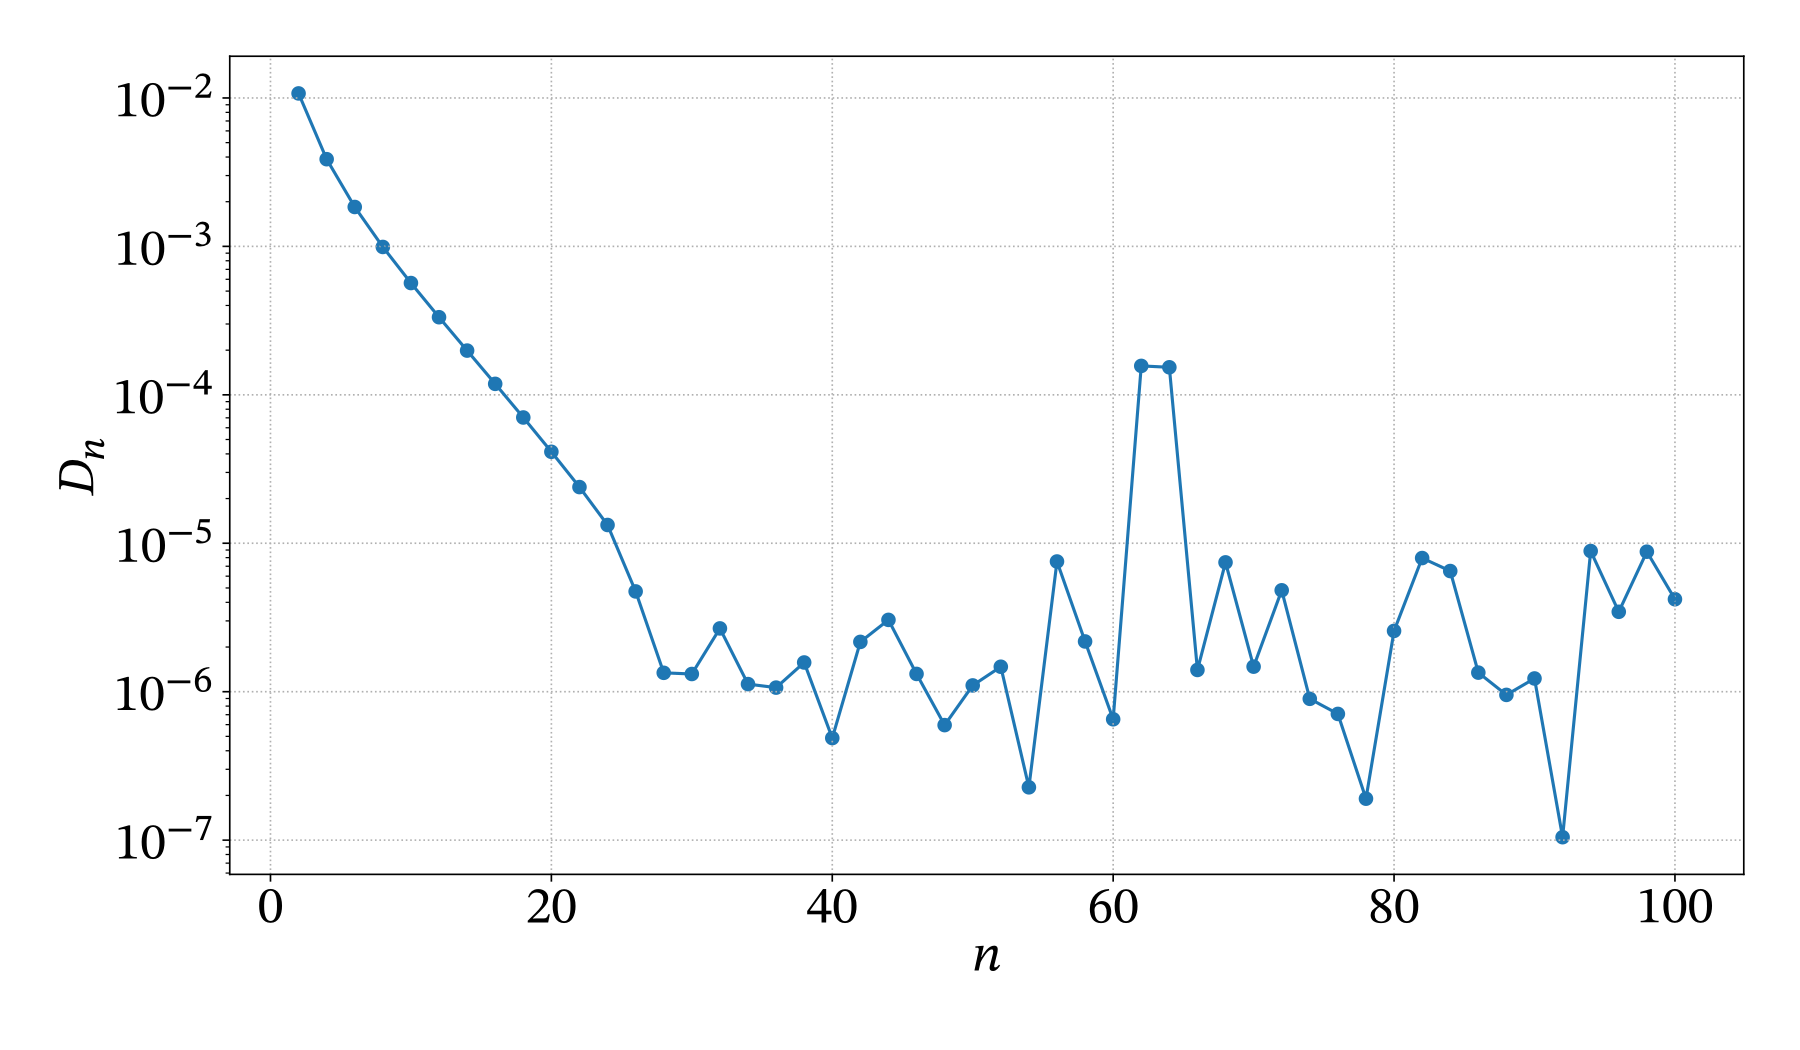
\includegraphics[width=\linewidth]{figures/Dn.png}
    \caption{Wartości $D_n$ dla wyższych $n$}
    \label{anom}
\end{figure}

\end{document}
